\documentclass[11pt,border=4pt]{standalone}
% Estilo comum dos fluxogramas do Caderno C3 (cores do modelo do MOP)
\usepackage[T1]{fontenc}
\usepackage[utf8]{inputenc}
\usepackage{helvet}
\renewcommand{\familydefault}{\sfdefault}
\usepackage{amssymb}
\usepackage{tikz}
\usetikzlibrary{positioning, arrows.meta, shapes.geometric, shapes.symbols, shapes.misc,
  calc, fit, backgrounds, decorations.pathmorphing, patterns, shadows}
% Paleta do modelo do caderno
\definecolor{cTeal}{HTML}{00747A}
\definecolor{cNavy}{HTML}{0B3A5A}
\definecolor{cBlue}{HTML}{0A73BA}
\definecolor{cBlueBg}{HTML}{EBF4F9}
\definecolor{cTealBg}{HTML}{E3F1F2}
\definecolor{cTealMid}{HTML}{9CCFD2}
\definecolor{cGrayBg}{HTML}{F2F2F2}
\definecolor{cGrayLine}{HTML}{BFBFBF}
\definecolor{cGrayText}{HTML}{595959}
\definecolor{cText}{HTML}{1A1A1A}
\definecolor{cAmber}{HTML}{B7791F}
\definecolor{cAmberBg}{HTML}{FDF3DC}
\definecolor{cGreen}{HTML}{3D7D3A}
\definecolor{cGreenBg}{HTML}{E8F2E4}
\color{cText}
\tikzset{
  every node/.style={font=\footnotesize, text=cText},
  etapa/.style={draw=cTeal, fill=cTealBg, rounded corners=2pt, align=center,
     inner sep=3.5pt, minimum height=0.85cm, text width=#1, line width=0.6pt},
  etapa/.default={3.2cm},
  marco/.style={draw=cNavy, fill=cNavy, rounded corners=2pt, align=center,
     inner sep=3.5pt, minimum height=0.85cm, text width=#1,
     font=\footnotesize\bfseries, text=white},
  marco/.default={3.2cm},
  marcoteal/.style={draw=cTeal, fill=cTeal, rounded corners=2pt, align=center,
     inner sep=3.5pt, minimum height=0.85cm, text width=#1,
     font=\footnotesize\bfseries, text=white},
  marcoteal/.default={3.2cm},
  externo/.style={draw=cGrayLine, fill=cGrayBg, rounded corners=2pt, align=center,
     inner sep=3.5pt, minimum height=0.85cm, text width=#1},
  externo/.default={3.2cm},
  produto/.style={draw=cTeal!70, fill=white, rounded corners=1pt, align=center,
     inner sep=2.5pt, minimum height=0.6cm, text width=#1, font=\scriptsize},
  produto/.default={2.4cm},
  decisao/.style={draw=cAmber, fill=cAmberBg, diamond, aspect=2, align=center,
     inner sep=1pt, font=\scriptsize, line width=0.6pt},
  correcao/.style={draw=cAmber, fill=cAmberBg, rounded corners=2pt, align=center,
     inner sep=3pt, minimum height=0.8cm, text width=#1, font=\scriptsize},
  correcao/.default={2.6cm},
  transversal/.style={draw=cBlue, fill=cBlueBg, dashed, rounded corners=2pt, align=center,
     inner sep=3.5pt, text width=#1, line width=0.6pt},
  transversal/.default={6cm},
  seta/.style={-{Stealth[length=2.2mm,width=1.8mm]}, line width=0.8pt, draw=cNavy},
  setaleve/.style={-{Stealth[length=1.8mm,width=1.5mm]}, line width=0.6pt, draw=cGrayText},
  setatracejada/.style={-{Stealth[length=2mm]}, line width=0.7pt, dashed, draw=cGrayText},
  rotulo/.style={font=\scriptsize\itshape, text=cGrayText, fill=white, inner sep=1pt},
  fase/.style={signal, signal to=east, signal from=west, draw=cTeal, fill=cTealBg,
     align=center, font=\scriptsize\bfseries, minimum height=1.05cm, text width=#1,
     inner sep=2pt},
  fase/.default={1.9cm},
  raia/.style={draw=cGrayLine, fill=cGrayBg, minimum width=#1, minimum height=0.9cm,
     anchor=north west},
  tituloraia/.style={font=\scriptsize\bfseries, text=cNavy, align=center, text width=1.75cm},
  cab/.style={font=\scriptsize\bfseries, text=white, fill=cNavy, align=center,
     inner sep=3pt, text width=#1, minimum height=0.6cm},
  cab/.default={3cm},
  bloco/.style={draw=cGrayLine, fill=cGrayBg, rounded corners=3pt},
}
% sem hifenização nas caixas dos fluxogramas
\AtBeginDocument{\hyphenpenalty=10000 \exhyphenpenalty=10000 \sloppy}

\begin{document}

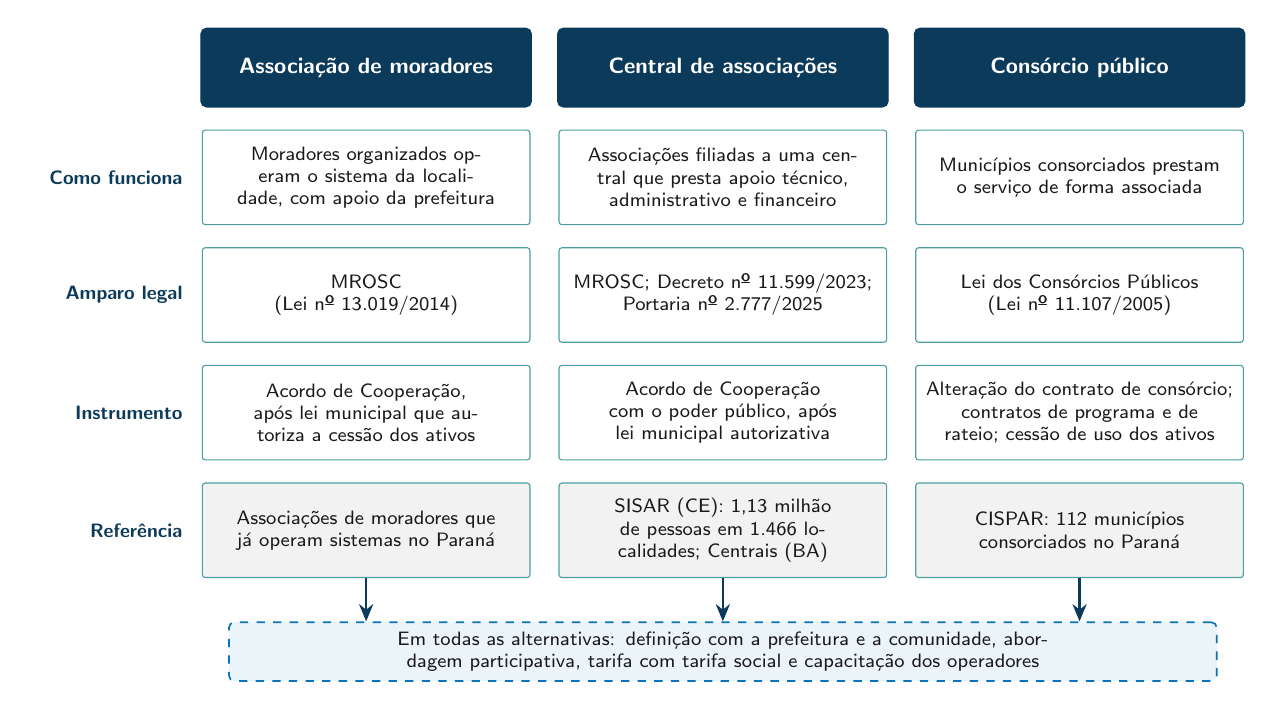
\begin{tikzpicture}[node distance=0.28cm,
    cel/.style={draw=cTeal!70, fill=white, align=center, font=\scriptsize,
                text width=3.95cm, minimum height=1.2cm, inner sep=3pt, rounded corners=1pt},
    rot/.style={font=\scriptsize\bfseries, text=cNavy, align=right, text width=1.85cm, anchor=east}]
  \node[marco=3.95cm, minimum height=1.0cm] (a0) at (0,0) {Associação de moradores};
  \node[marco=3.95cm, minimum height=1.0cm, right=0.32cm of a0] (b0) {Central de associações};
  \node[marco=3.95cm, minimum height=1.0cm, right=0.32cm of b0] (c0) {Consórcio público};

  \node[cel, below=of a0] (a1) {Moradores organizados operam o sistema da localidade, com apoio da prefeitura};
  \node[cel, below=of b0] (b1) {Associações filiadas a uma central que presta apoio técnico, administrativo e financeiro};
  \node[cel, below=of c0] (c1) {Municípios consorciados prestam o serviço de forma associada};

  \node[cel, below=of a1] (a2) {MROSC\\ (Lei nº 13.019/2014)};
  \node[cel, below=of b1] (b2) {MROSC; Decreto nº 11.599/2023;\\ Portaria nº 2.777/2025};
  \node[cel, below=of c1] (c2) {Lei dos Consórcios Públicos\\ (Lei nº 11.107/2005)};

  \node[cel, below=of a2] (a3) {Acordo de Cooperação, após lei municipal que autoriza a cessão dos ativos};
  \node[cel, below=of b2] (b3) {Acordo de Cooperação com o poder público, após lei municipal autorizativa};
  \node[cel, below=of c2] (c3) {Alteração do contrato de consórcio; contratos de programa e de rateio; cessão de uso dos ativos};

  \node[cel, fill=cGrayBg, below=of a3] (a4) {Associações de moradores que já operam sistemas no Paraná};
  \node[cel, fill=cGrayBg, below=of b3] (b4) {SISAR (CE): 1,13 milhão de pessoas em 1.466 localidades; Centrais (BA)};
  \node[cel, fill=cGrayBg, below=of c3] (c4) {CISPAR: 112 municípios consorciados no Paraná};

  \node[rot] at ($(a1.west)+(-0.12,0)$) {Como funciona};
  \node[rot] at ($(a2.west)+(-0.12,0)$) {Amparo legal};
  \node[rot] at ($(a3.west)+(-0.12,0)$) {Instrumento};
  \node[rot] at ($(a4.west)+(-0.12,0)$) {Referência};

  \node[transversal=12.3cm, below=0.55cm of b4, font=\scriptsize] (r) {Em todas as alternativas: definição com a prefeitura
    e a comunidade, abordagem participativa, tarifa com tarifa social e capacitação dos operadores};
  \foreach \n in {a4, b4, c4} \draw[seta] (\n) -- (\n |- r.north);
\end{tikzpicture}

\end{document}
